\documentclass[tikz,border=2pt]{standalone}
% Preámbulo común de los diagramas TikZ (misma paleta y letra que las notas)
\usepackage[T1]{fontenc}\usepackage[utf8]{inputenc}
\usepackage{libertinus}\usepackage{libertinust1math}
\usepackage[defaultsans,scale=0.92]{lato}
\usepackage{amsmath,amssymb,bm}
\usepackage{tikz}\usetikzlibrary{calc,positioning,arrows.meta,shapes.geometric,decorations.pathreplacing,decorations.pathmorphing,fit,backgrounds}
\definecolor{snlazul}{HTML}{1E5AA8}\definecolor{snlnoche}{HTML}{14213D}\definecolor{snlvioleta}{HTML}{6C4AB6}
\definecolor{snlcoral}{HTML}{D1495B}\definecolor{snlambar}{HTML}{E09F3E}\definecolor{snlverde}{HTML}{2A9D8F}
\definecolor{snlteal}{HTML}{0F7173}\definecolor{snlgris}{HTML}{5C677D}\definecolor{snlfondo}{HTML}{F4F6FA}
\tikzset{>={Stealth[length=2.2mm]},
  bloque/.style={draw=#1,fill=#1!8,thick,rounded corners=2pt,minimum height=11mm,minimum width=20mm,align=center,font=\small},
  bloque/.default=snlazul,
  suma/.style={draw=snlnoche,thick,circle,inner sep=0pt,minimum size=5mm},
  flecha/.style={->,thick,draw=snlnoche},
  etq/.style={font=\small,text=snlnoche},
  nota/.style={font=\footnotesize\sffamily,text=snlgris,align=center}}

\begin{document}
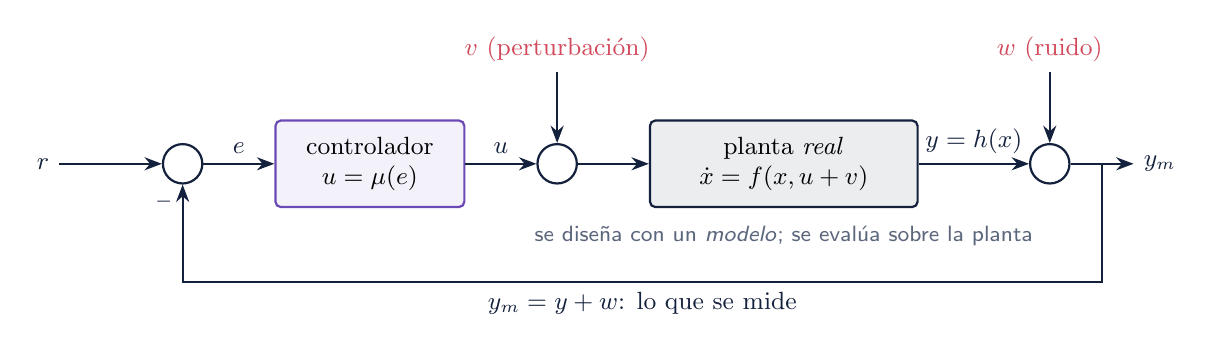
\begin{tikzpicture}
 \node[suma] (s0) {};
 \node[bloque=snlvioleta,right=9mm of s0,minimum width=24mm] (K) {controlador\\$u=\mu(e)$};
 \node[suma,right=9mm of K] (s1) {};
 \node[bloque=snlnoche,right=9mm of s1,minimum width=34mm] (P) {planta \emph{real}\\$\dot x=f(x,u+v)$};
 \node[suma,right=14mm of P] (s2) {};
 \draw[flecha] ($(s0.west)+(-13mm,0)$) node[left,etq]{$r$} -- (s0);
 \draw[flecha] (s0) -- node[above,etq]{$e$} (K);
 \draw[flecha] (K) -- node[above,etq]{$u$} (s1);
 \draw[flecha] ($(s1.north)+(0,9mm)$) node[above,etq,text=snlcoral]{$v$ (perturbación)} -- (s1);
 \draw[flecha] (s1) -- (P);
 \draw[flecha] (P) -- node[above,etq]{$y=h(x)$} (s2);
 \draw[flecha] ($(s2.north)+(0,9mm)$) node[above,etq,text=snlcoral]{$w$ (ruido)} -- (s2);
 \draw[flecha] (s2.east) -- ++(8mm,0) node[right,etq]{$y_m$};
 \draw[flecha] ($(s2.east)+(4mm,0)$) -- ++(0,-15mm) -| node[pos=0.25,below,etq]{$y_m=y+w$: lo que se mide} (s0.south);
 \node[font=\scriptsize,text=snlnoche] at ($(s0.south)+(-2.4mm,-2.2mm)$) {$-$};
 \node[nota,below=1mm of P] {se diseña con un \emph{modelo}; se evalúa sobre la planta};
\end{tikzpicture}
\end{document}
